% AUTO-GENERATED by writeup/make_rehaul_ladder.py -- do not edit; re-run the script.
% Figure fig:rh_ladder (Section 8): the feature-count ladder, results/ladder_2026-10-26 (RULE.txt sections 1-6).
\begin{figure}[tbp]
  \centering
  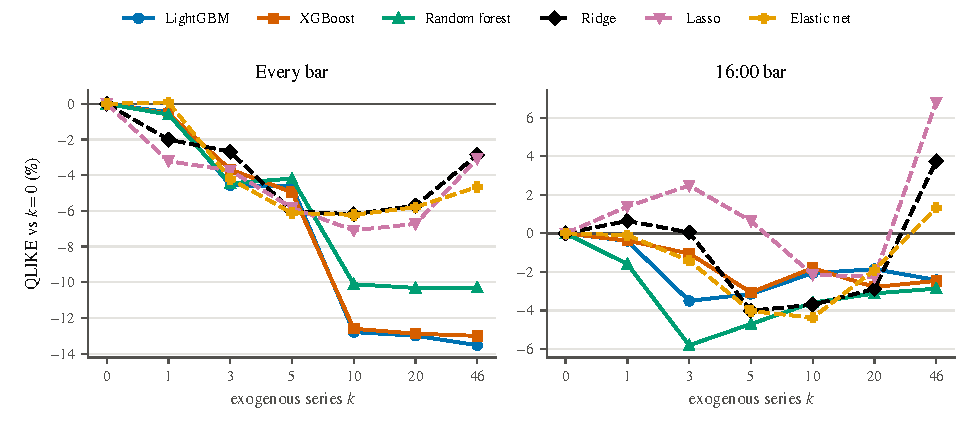
\includegraphics[width=\linewidth]{figures/rehaul_ladder.pdf}
  \caption{How many exogenous series carry the gain. Each model is refitted on its top $k$ exogenous series only
    ($k = 0$ is the HAR benchmark set, $k = \rhldNSeries$ the full set), ranked once by the model's own importance
    measure on a fit explained on \rhldRankYear{} data, before the evaluation span. Vertical axis: the QLIKE of the
    rung relative to the same model's $k = 0$ rung, in percent (negative: more accurate), on the \rhldNBars{} bars
    of Table~\ref{tab:rh_oos} (left) and on their 16:00 bar (right). Monthly refits at \rhldNOrigins{} origins, each
    held for \rhldHoldSessions{} sessions, window $W = \rhldWindowDays$ trading days, hyperparameters frozen.
    Pre-patch design: the FOMC calendar features before the fix of Section~\ref{sec:rh_data}.}
  \label{fig:rh_ladder}
\end{figure}
